% Lean-certified finite-dimensional complex Schatten transport theorem.
\section{Exact Schatten costs for complex subspace transport}
\label{sec:schatten-optimization}

Fix $1<p<2$. For $0\leq t\leq\pi$, set
\[
 f_p(t)=\bigl(2\sin(t/2)\bigr)^p,
 \qquad
 a_p(t)=\cos(t/2)\bigl(2\sin(t/2)\bigr)^{p-1},
 \qquad
 \vartheta_p=\arccos\frac{2-p}{p}.
\]
Thus $f_p'=p a_p$ on $(0,\pi)$ and $0<\vartheta_p<\pi/2$.
For a principal angle $\theta\in[0,\pi/2]$, define
\begin{equation}
 m_p(\theta)=\min_{0\leq\delta\leq\theta}
       \{f_p(\theta+\delta)+f_p(\theta-\delta)\}.
 \label{eq:schatten-plane-cost}
\end{equation}
Multiplying a planar direct rotation by $e^{i\delta}$ changes its two
eigenphases from $(\theta,-\theta)$ to $(\theta+\delta,-\theta+\delta)$.
The expression in \cref{eq:schatten-plane-cost} is its full displacement
Schatten power sum.

Bolotnikov, Li, and Rodman \citep[Lemmas~3.2--3.3]{bolotnikov2001minimal}
solve the planar problem for $p\geq2$ and the right-angle case for
$1\leq p<2$. Their general constrained problem also includes subspace
transport. The following scalar classification supplies the dependence on
the angle in the remaining exponent range.

\begin{proposition}[The scalar phase diagram]
\label{prop:schatten-scalar-diagram}
The minimum in \cref{eq:schatten-plane-cost} has the following description.
\begin{enumerate}
 \item If $0\leq\theta\leq\vartheta_p$, its unique minimizing phase is
 $\delta=0$, and $m_p(\theta)=2f_p(\theta)$. Its phase derivative is
 strictly positive on $(0,\theta)$.
 \item If $\vartheta_p<\theta<\pi/2$, its unique minimizing phase
 $\delta_p(\theta)$ is the unique solution in $(0,\theta)$ of
 \begin{equation}
    a_p(\theta+\delta)=a_p(\theta-\delta).
    \label{eq:schatten-stationary-balance}
 \end{equation}
 \item At $\theta=\pi/2$, the unique minimizing phase is $\delta=\theta$,
 and $m_p(\pi/2)=2^p$.
\end{enumerate}
\end{proposition}

\begin{proof}
For $0\leq\delta<\theta<\pi/2$, both amplitudes in
\cref{eq:schatten-stationary-balance} are positive. Their logarithmic ratio
\[
 D_{p,\theta}(\delta)=
       \log a_p(\theta+\delta)-\log a_p(\theta-\delta)
\]
has the same sign as the derivative of the objective in
\cref{eq:schatten-plane-cost}. Direct differentiation gives
\begin{equation}
 D_{p,\theta}'(\delta)=
 \frac{\sin\theta\,[p\cos\theta-(2-p)\cos\delta]}
      {\cos^2\delta-\cos^2\theta}.
 \label{eq:schatten-log-ratio-derivative}
\end{equation}
The denominator is positive on $(0,\theta)$, and the bracket in the
numerator increases strictly there. If $\theta\leq\vartheta_p$, that
bracket is positive for every $\delta>0$, including when it vanishes at
$\delta=0$. Since $D_{p,\theta}(0)=0$, the objective increases strictly
on $[0,\theta]$.

If $\theta>\vartheta_p$, the bracket starts negative and ends positive.
Consequently $D_{p,\theta}$ first decreases and then increases. Moreover,
$D_{p,\theta}(\delta)\to+\infty$ as $\delta\uparrow\theta$, because
$a_p(2\theta)>0$ and $a_p(0)=0$. It has exactly one positive zero, and
the objective decreases before that zero and increases afterward.
Continuity includes the endpoint $\delta=\theta$.

For $\theta=\pi/2$, \cref{eq:schatten-log-ratio-derivative} becomes
$D_{p,\pi/2}'(\delta)=-(2-p)/\cos\delta<0$. The objective therefore
decreases strictly up to its endpoint, where its two displacement singular
values are $2$ and $0$. The case $\theta=0$ has only one admissible phase.
\end{proof}

\begin{figure}[t]
 \centering
 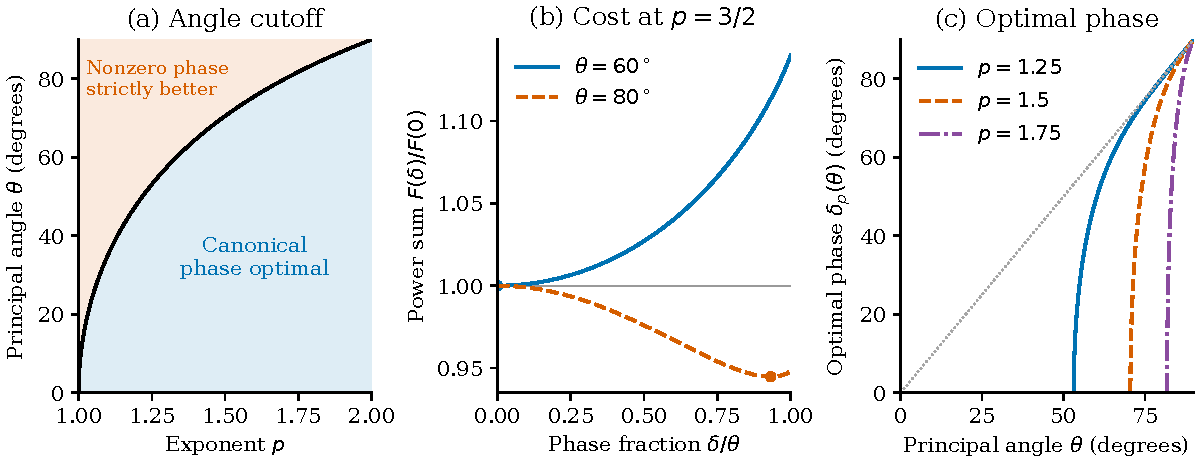
\includegraphics[width=\linewidth]{figures/schatten_phase_diagram.pdf}
 \caption{The scalar phase transition. The cutoff is
 $\vartheta_p=\arccos((2-p)/p)$. At $p=3/2$, the canonical phase minimizes
 the cost at $60^\circ$, while an interior phase gives a smaller cost at
 $80^\circ$. The optimizing phase starts at zero and approaches the
 principal angle at the right-angle boundary.}
 \label{fig:schatten-phase-diagram}
\end{figure}

The scalar minimization determines the unrestricted complex problem as well.
Write $\mathcal U(P,Q)=\{W\in U(n):WPW^*=Q\}$ for the transporters of
two orthogonal projections of equal rank.

\begin{proposition}[The unrestricted planar minimum]
\label{prop:schatten-planar-minimum}
For two complex lines of principal angle $\theta$ in $\mathbb C^2$,
the minimum displacement power over all unitary transporters is
$m_p(\theta)$.
\end{proposition}

\begin{proof}
Let $x$ be a unit vector in the source line. For an admissible $W$,
$|\langle x,Wx\rangle|=\cos\theta$. Write its eigenphases in
$[-\pi,\pi]$ as $\alpha,\beta$. In an orthonormal eigenbasis,
\[
 \langle x,Wx\rangle=s e^{i\alpha}+(1-s)e^{i\beta},\qquad 0\leq s\leq1.
\]
Multiplying this average by $e^{-i(\alpha+\beta)/2}$ gives real part
$\cos((\alpha-\beta)/2)$. If $|\alpha|+|\beta|<2\theta$, its modulus
would consequently be at least
$\cos((|\alpha|+|\beta|)/2)>\cos\theta$, a contradiction. Thus
$|\alpha|+|\beta|\geq2\theta$.

Scale the two nonnegative absolute eigenphases down, if necessary, until
their sum is $2\theta$. Both remain in $[0,\pi]$, where $f_p$ increases.
Reordering the resulting angles gives $\theta+\delta,\theta-\delta$
for some $0\leq\delta\leq\theta$. Hence
\[
 \|I-W\|_p^p=f_p(|\alpha|)+f_p(|\beta|)
       \geq f_p(\theta+\delta)+f_p(\theta-\delta)\geq m_p(\theta).
\]
The zero total-angle case has $\theta=0$ and the same conclusion.
An optimizing scalar phase attains the bound.
\end{proof}

\begin{theorem}[Independent principal-plane minimization]
\label{thm:schatten-independent-planes}
Let $P,Q$ be orthogonal projections of rank $r$ on $\mathbb C^n$, and let
$\theta_1,\ldots,\theta_r\in[0,\pi/2]$ be their principal angles, with
multiplicity. Then
\begin{equation}
 \boxed{\min_{W\in\mathcal U(P,Q)}\|I-W\|_p^p
                 =\sum_{j=1}^r m_p(\theta_j).}
 \label{eq:schatten-unrestricted-minimum}
\end{equation}
An attaining transporter is the identity on the fixed summands of a
cosine--sine decomposition and, on each nonzero principal plane, a scalar
phase of the direct rotation with phase $\delta_p(\theta_j)$ or its
negative. In particular, allowing transports that mix principal planes
cannot lower the minimum.
\end{theorem}


\begin{lstlisting}[style=leanpaper,
 caption={Lean signature for the unrestricted Schatten minimum. The surrounding
 finite-dimensional complex Hilbert-space context is omitted. The parameter
 \texttt{p} is an extended nonnegative real; the hypotheses require its finite
 real value to lie in $(1,2)$. The scalar minimum is \texttt{phaseMinimum}.},
 label={lst:schatten-global}]
theorem exists_unitary_minimizing_schatten_transport_principalAngles
    (p : ENNReal) [Fact (1 <= p)] (hp : p != ⊤)
    (hp1 : 1 < p.toReal) (hp2 : p.toReal < 2)
    (K L : Submodule Complex E)
    (hKL : Module.finrank Complex K = Module.finrank Complex L) :
    ∃ W : LinearIsometryEquiv (RingHom.id Complex) E E,
      K.map W.toLinearMap = L ∧
      UnitarilyInvariantSeminorm.schatten Complex E E p
          (LinearMap.id - W.toLinearMap) ^ p.toReal =
        (Finset.univ.sum (fun i : Fin (Module.finrank Complex K) =>
          phaseMinimum p.toReal (K.principalAngles L i))) ∧
      ∀ T : LinearIsometryEquiv (RingHom.id Complex) E E,
        K.map T.toLinearMap = L ->
        (Finset.univ.sum (fun i : Fin (Module.finrank Complex K) =>
          phaseMinimum p.toReal (K.principalAngles L i))) <=
          UnitarilyInvariantSeminorm.schatten Complex E E p
            (LinearMap.id - T.toLinearMap) ^ p.toReal
\end{lstlisting}

We give the reduction to principal planes before proving the theorem.
Extend the scalar cost to the $2\pi$-periodic function
\[
 \phi_p(t)=\bigl(2|\sin(t/2)|\bigr)^p.
\]
It is continuously differentiable because $p>1$. If
$W=\sum_j e^{it_j}E_j$ is a spectral decomposition of a unitary, put
\[
 G_p(W)=\sum_j\phi_p'(t_j)E_j.
\]
The definition is independent of the phase representatives. This
self-adjoint operator commutes with $W$.

\begin{proposition}[First variation and two spectral roots]
\label{prop:schatten-critical-blocks}
If $W$ is a local minimum of the displacement power on $\mathcal U(P,Q)$ and
$J=2P-I$, then
\begin{equation}
 JG_p(W)J=-G_p(W).
 \label{eq:schatten-gradient-anticommutation}
\end{equation}
For each positive eigenvalue $g$ of $G_p(W)$, the spaces $H_g$ and
$H_{-g}$ have the same dimension. Identifying them by $J$, the restriction
of $W$ to their sum has the form
\begin{equation}
 W_+=e^{ia}\exp\bigl(i(b-a)A\bigr),\qquad
 W_-=e^{-ia}\exp\bigl(-i(b-a)B\bigr),
 \label{eq:schatten-critical-two-roots}
\end{equation}
where $A,B$ are orthogonal projections on $H_g$ and
\[
 0<a<\vartheta_p<b<\pi,\qquad p a_p(a)=p a_p(b)=g.
\]
When $g=p a_p(\vartheta_p)$, both restrictions instead have the single
eigenphase $\vartheta_p$ and $-\vartheta_p$, respectively.
\end{proposition}

\begin{proof}
For a Hermitian $H$ commuting with $P$, the curve $W\exp(itH)$ remains
in $\mathcal U(P,Q)$. The spectral first-derivative formula gives
\begin{equation}
 \left.\frac{d}{dt}\|I-W\exp(itH)\|_p^p\right|_{t=0}
              =\operatorname{tr}(G_p(W)H).
 \label{eq:schatten-first-variation}
\end{equation}
For completeness, choose a local logarithm of the unitary near $W$ with
its cut outside the finite spectrum. Apply the differentiability theorem
for Hermitian spectral functions \citep[Theorem~1.1]{lewis1996derivatives}
to the resulting Hermitian logarithm. In an eigenbasis, differentiating
$W\exp(itH)$ shows that the diagonal entries of the logarithm's derivative
are those of $H$, which gives \cref{eq:schatten-first-variation}.
The derivative vanishes for every such $H$. Taking $H$ supported on
either diagonal block relative to $P\oplus P^\perp$ shows that the two
diagonal compressions of $G_p(W)$ vanish. This is
\cref{eq:schatten-gradient-anticommutation}.

The operator $J$ therefore interchanges $H_g$ and $H_{-g}$. On their sum
we can write $J=\left(\begin{smallmatrix}0&I\\I&0\end{smallmatrix}\right)$.
Since $W$ commutes with $G_p(W)$, it is block diagonal there. On
$(0,\pi)$,
\begin{equation}
 a_p'(t)=\frac12\bigl(2\sin(t/2)\bigr)^{p-2}
                    [p\cos t-(2-p)].
 \label{eq:schatten-amplitude-derivative}
\end{equation}
Thus $a_p$ increases strictly up to $\vartheta_p$ and decreases strictly
afterward, with zero endpoint values. The equation $p a_p(t)=g$ has
exactly the two stated roots, except at its maximum, where the roots
coincide. The signs of $\phi_p'$ distinguish the positive and negative
phase spaces and give \cref{eq:schatten-critical-two-roots}.
\end{proof}

\begin{lemma}[Second variation on a two-phase block]
\label{lem:schatten-two-phase-hessian}
Let $\alpha,\beta\in(-\pi,\pi)\setminus\{0\}$ be distinct and satisfy
$\phi_p'(\alpha)=\phi_p'(\beta)$. For an orthogonal projection $A$, put
$V=e^{i\alpha}(I-A)+e^{i\beta}A$. If $X=X^*$, then
\begin{align}
 \left.\frac{d^2}{dt^2}\|I-V\exp(itX)\|_p^p\right|_{t=0}
  &=\phi_p''(\alpha)\|(I-A)X(I-A)\|_2^2
    +\phi_p''(\beta)\|AXA\|_2^2.
 \label{eq:schatten-two-phase-hessian}
\end{align}
Here $\|\cdot\|_2$ is the Frobenius norm.
\end{lemma}

\begin{proof}
Choose a smooth Hermitian logarithm $L(t)$ of $V\exp(itX)$ near zero,
with $L(0)=\alpha(I-A)+\beta A$. The spectral trace Hessian formula
\citep[Theorem~3.3]{lewis2001twice} applies to the sum of the scalar
function $\phi_p$ near these two nonzero phases. Its Hermitian version
follows from the real symmetric version by realification, which doubles
both spectral traces. Since the two scalar first derivatives agree, the
cross terms between distinct eigenspaces vanish. The second derivative
along $L(t)$ is therefore
\[
 \phi_p''(\alpha)\|(I-A)L'(0)(I-A)\|_2^2
 +\phi_p''(\beta)\|AL'(0)A\|_2^2
 +\phi_p'(\alpha)\operatorname{tr}L''(0).
\]
Differentiate $\exp(iL(t))=V\exp(itX)$ and compress to its initial
eigenspaces. The exponential power series gives
\[
 AL'(0)A=AXA,\qquad
 (I-A)L'(0)(I-A)=(I-A)X(I-A).
\]
Finally,
\[
 \exp(i\operatorname{tr}L(t))=\det(V)\exp(it\operatorname{tr}X).
\]
Continuity fixes the integer ambiguity, so $\operatorname{tr}L(t)$ is
affine near zero and its second derivative vanishes. This proves the
formula.
\end{proof}

\begin{proposition}[Exclusion of overlapping large-phase spaces]
\label{prop:schatten-no-mixing}
At a local minimum, the two large-phase projections in
\cref{eq:schatten-critical-two-roots} satisfy $AB=0$.
\end{proposition}

\begin{proof}
Suppose $AB\ne0$ and set
\begin{equation}
 X=AB+BA.
 \label{eq:schatten-mixing-direction}
\end{equation}
This operator is Hermitian, and idempotence gives
\[
 (I-A)X(I-A)=(I-B)X(I-B)=0,\qquad
 AXA=2ABA,\quad BXB=2BAB.
\]
Use the same $X$ on $H_g$ and $H_{-g}$ and zero on the remaining
blocks. The resulting Hermitian $H=\operatorname{diag}(X,X)$ commutes
with $J$, so $W\exp(itH)$ is feasible.

Apply \cref{lem:schatten-two-phase-hessian} to $W_+$ and $W_-$.
Their phase derivatives are constant on each block, and $\phi_p''$ is
even. The complementary compressions vanish, leaving
\begin{equation}
 \left.\frac{d^2}{dt^2}\|I-W\exp(itH)\|_p^p\right|_{t=0}
     =4f_p''(b)\bigl(\|ABA\|_2^2+\|BAB\|_2^2\bigr)<0.
 \label{eq:schatten-mixing-negative-curvature}
\end{equation}
Indeed, $f_p''(b)=p a_p'(b)<0$ because $b>\vartheta_p$.
Also $ABA=(BA)^*(BA)$, so $AB\ne0$ implies $ABA\ne0$.
Thus the displayed squared-norm sum is positive. All other spectral
blocks stay fixed along the curve, so zero displacement singular values
there do not affect this second derivative. The negative second variation
contradicts local minimality, proving $AB=0$.
\end{proof}

\begin{proof}[Proof of \cref{thm:schatten-independent-planes}]
The feasible set is nonempty and compact, so a minimum exists. Choose a
minimizer $W$ and decompose by the eigenspaces of $G_p(W)^2$. These
spaces reduce $P$, $W$, and $Q=WPW^*$.

Consider a nonzero spectral block. When the amplitude roots coincide,
it is a sum of canonical planes with angle $\vartheta_p$. Otherwise,
\cref{prop:schatten-no-mixing} gives the orthogonal decomposition
\[
 H_g=\operatorname{ran}A\oplus\operatorname{ran}B
              \oplus(\ker A\cap\ker B).
\]
The common kernel produces canonical planes of angle $a$, each with
cost $2f_p(a)=m_p(a)$. Each of the other two summands produces a plane
with eigenphases $(b,-a)$ or $(a,-b)$.

Put $\sigma=(a+b)/2$. We have $a+b<\pi$: indeed,
\[
 \frac{a_p(\pi-a)}{a_p(a)}
        =\tan(a/2)^{2-p}<1,
\]
and $a_p$ decreases strictly on $(\vartheta_p,\pi)$. The phase
$(b-a)/2$ satisfies \cref{eq:schatten-stationary-balance} for
$\theta=\sigma$, so \cref{prop:schatten-scalar-diagram} implies
$\sigma>\vartheta_p$ and $f_p(a)+f_p(b)=m_p(\sigma)$.
To identify the geometric angle, note that on $H_g\oplus H_{-g}$,
\[
 (2Q-I)(2P-I)=
 \operatorname{diag}(W_+W_-^*,W_-W_+^*).
\]
Its scalar phases on the displayed summands are $\pm2a$ or
$\pm(a+b)$, so their principal angles are exactly $a$ or $\sigma$.
The cost on every nonzero spectral block is consequently the sum of
the corresponding $m_p$ costs.

On $\ker G_p(W)$ the unitary has only eigenvalues $1$ and $-1$.
Its displacement singular values are consequently zero or two. The
projection-distance inequality gives
\[
 \|I-W\|_p^p
   =2^{p-1}\|I-W\|_1
   \geq2^{p-1}\|P-Q\|_1
   =2^p\sum_j\sin\theta_j.
\]
For every physical angle,
$m_p(\theta)\leq(2\sin\theta)^p\leq2^p\sin\theta$, using
$p>1$ and $0\leq\sin\theta\leq1$. This block therefore also costs at
least the sum of its principal-plane minima. Combining the blocks gives
the lower inequality in \cref{eq:schatten-unrestricted-minimum}.

For the reverse inequality, use a cosine--sine decomposition of $P,Q$.
On each nonzero principal plane choose the scalar phase from
\cref{prop:schatten-scalar-diagram}, and use the identity on the remaining
fixed space. The orthogonal sum is an admissible unitary. Schatten
power sums add across these blocks, giving exactly the right-hand side
of \cref{eq:schatten-unrestricted-minimum}.
\end{proof}


\begin{corollary}[The canonical cutoff]
\label{cor:schatten-canonical-cutoff}
The canonical rotation, completed by right-angle rotations when necessary,
is globally minimizing if and only if every principal angle satisfies
$\theta_j\leq\vartheta_p$. If any angle exceeds this cutoff, an
independently phase-modified transport has strictly smaller cost.
\end{corollary}

\begin{proof}
The canonical displacement power is $\sum_j 2f_p(\theta_j)$.
Each scalar minimum is at most its canonical cost, with equality precisely
for $\theta_j\leq\vartheta_p$ by the scalar classification, including
zero and right angles. Apply \cref{thm:schatten-independent-planes} and
sum these nonnegative differences.
\end{proof}

The proof turns the failure of universal direct-rotation minimality into
an exact decision and construction. A cosine--sine decomposition supplies
the principal planes. The canonical phase suffices below the cutoff;
above it a single scalar equation with a unique interior root determines
the phase, and at a right angle the endpoint phase attains the minimum.
The lower bound certifies optimality against all ambient unitary transports.
